\documentclass{article}

% if you need to pass options to natbib, use, e.g.:
%     \PassOptionsToPackage{numbers, compress}{natbib}
% before loading neurips_2026

% The authors should use one of these tracks.
% Before accepting by the NeurIPS conference, select one of the options below.
% 0. "default" for submission
\usepackage{neurips_2026}
% the "default" option is equal to the "main" option, which is used for the Main Track with double-blind reviewing.
% 1. "main" option is used for the Main Track
%  \usepackage[main]{neurips_2026}
% 2. "position" option is used for the Position Paper Track
%  \usepackage[position]{neurips_2026}
% 3. "eandd" option is used for the Evaluations & Datasets Track
 % \usepackage[eandd]{neurips_2026}
 % if you need to opt-in for a single-blind submission in the E&D track:
 %\usepackage[eandd, nonanonymous]{neurips_2026}
% 4. "creativeai" option is used for the Creative AI Track
%  \usepackage[creativeai]{neurips_2026}
% 5. "sglblindworkshop" option is used for the Workshop with single-blind reviewing
 % \usepackage[sglblindworkshop]{neurips_2026}
% 6. "dblblindworkshop" option is used for the Workshop with double-blind reviewing
%  \usepackage[dblblindworkshop]{neurips_2026}

% After being accepted, the authors should add "final" behind the track to compile a camera-ready version.
% 1. Main Track
 % \usepackage[main, final]{neurips_2026}
% 2. Position Paper Track
%  \usepackage[position, final]{neurips_2026}
% 3. Evaluations & Datasets Track
 % \usepackage[eandd, final]{neurips_2026}
% 4. Creative AI Track
%  \usepackage[creativeai, final]{neurips_2026}
% 5. Workshop with single-blind reviewing
%  \usepackage[sglblindworkshop, final]{neurips_2026}
% 6. Workshop with double-blind reviewing
%  \usepackage[dblblindworkshop, final]{neurips_2026}
% Note. For the workshop paper template, both \title{} and \workshoptitle{} are required, with the former indicating the paper title shown in the title and the latter indicating the workshop title displayed in the footnote.
% For workshops (5., 6.), the authors should add the name of the workshop, "\workshoptitle" command is used to set the workshop title.
% \workshoptitle{WORKSHOP TITLE}

% "preprint" option is used for arXiv or other preprint submissions
 % \usepackage[preprint]{neurips_2026}

% to avoid loading the natbib package, add option nonatbib:
%    \usepackage[nonatbib]{neurips_2026}

\usepackage[utf8]{inputenc} % allow utf-8 input
\usepackage[T1]{fontenc}    % use 8-bit T1 fonts
\usepackage{hyperref}       % hyperlinks
\usepackage{url}            % simple URL typesetting
\usepackage{booktabs}       % professional-quality tables
\usepackage{amsfonts}       % blackboard math symbols
\usepackage{nicefrac}       % compact symbols for 1/2, etc.
\usepackage{microtype}      % microtypography
\usepackage{xcolor}         % colors

\usepackage{amsmath}
\usepackage{amssymb}
\usepackage{graphicx}

% Note. For the workshop paper template, both \title{} and \workshoptitle{} are required, with the former indicating the paper title shown in the title and the latter indicating the workshop title displayed in the footnote. 
\title{Align to Retrieve: Multi-Scale Semantic Latent Alignment for Retrieval-Augmented Text-to-Motion Generation}

% The \author macro works with any number of authors. There are two commands
% used to separate the names and addresses of multiple authors: \And and \AND.
%
% Using \And between authors leaves it to LaTeX to determine where to break the
% lines. Using \AND forces a line break at that point. So, if LaTeX puts 3 of 4
% authors names on the first line, and the last on the second line, try using
% \AND instead of \And before the third author name.


\author{%
  David S.~Hippocampus\thanks{Use footnote for providing further information
    about author (webpage, alternative address)---\emph{not} for acknowledging
    funding agencies.} \\
  Department of Computer Science\\
  Cranberry-Lemon University\\
  Pittsburgh, PA 15213 \\
  \texttt{hippo@cs.cranberry-lemon.edu} \\
  % examples of more authors
  % \And
  % Coauthor \\
  % Affiliation \\
  % Address \\
  % \texttt{email} \\
  % \AND
  % Coauthor \\
  % Affiliation \\
  % Address \\
  % \texttt{email} \\
  % \And
  % Coauthor \\
  % Affiliation \\
  % Address \\
  % \texttt{email} \\
  % \And
  % Coauthor \\
  % Affiliation \\
  % Address \\
  % \texttt{email} \\
}


\begin{document}


\maketitle


\begin{abstract}
Text-to-motion generation (T2M) aims to synthesize realistic 3D human motion sequences conditioned on natural language descriptions.
Recent latent-space methods such as MotionStreamer~\citep{xiao2025motionstreamer} achieve strong motion fidelity,
but their encoders are optimized exclusively for reconstruction:
the resulting latent space is semantically unstructured, forcing text-motion alignment entirely onto the second-stage generator---which degrades for complex or compositional descriptions---
and preventing the latent space from serving as a retrieval index for real motion priors.
Our key insight is that organizing the motion latent space at multiple semantic scales lets it simultaneously act as a structured generation prior and a discriminative retrieval index,
making alignment, retrieval, and generation mutually reinforcing rather than disjoint modules.
To this end, we propose \textbf{MSA-T2M}, built on two tightly coupled components.
\textbf{MSA-VAE} is a causal variational autoencoder that performs joint local-global semantic alignment,
producing a latent space that explicitly encodes both fine-grained frame-level action semantics and high-level compositional sequence intent.
Building on this aligned space, \textbf{RAG-Diffusion-AR} retrieves semantically precise motion priors from the aligned latent bank and injects them into an autoregressive diffusion Transformer via Synergistic Classifier-Free Guidance,
yielding more discriminative priors than existing raw-space retrieval methods~\citep{zhang2023remodiffuse,kalakonda2025morag}.
Experiments on HumanML3D-272 show that MSA-T2M achieves the best FID (10.832) among all methods,
with ablations confirming the independent contributions of multi-scale alignment and retrieval augmentation.
\end{abstract}


\section{Introduction}

Text-driven human motion generation (T2M) plays a central role in applications such as virtual reality, animation, and embodied AI \citep{Guo_2022_CVPR,tevet2022human,xiao2025motionstreamer}.
Recent advances have progressively shifted from discrete VQ-VAE-based tokenization \citep{zhang2023generating} to continuous latent-space generation \citep{meng2024rethinking,meng2025absolute,xiao2025motionstreamer}, where causally-structured compact representations better preserve motion fidelity and enable high-quality sequential synthesis.
However, these latent spaces are optimized exclusively for motion reconstruction: semantic information is entangled with physical dynamics and remains unstructured.
Without explicit semantic organization in the latent space, text-motion alignment is delegated entirely to the second-stage generator and degrades sharply for complex or compositional descriptions.

The value of a semantically structured motion representation has long been recognized.
MotionCLIP \citep{tevet2022motionclip} pioneered cross-modal alignment by pulling motion encoder outputs toward CLIP text embeddings, yielding strong semantic interpretability.
Yet, subsequent state-of-the-art methods \citep{tevet2022human,chen2023executing,zhang2023generating,xiao2025motionstreamer} gradually abandoned explicit latent-space alignment, delegating text-motion correspondence entirely to the second-stage generator.
The few works that revisit latent-space alignment \citep{he2025molingo,yu2026causal} impose only single-scale, frame-level local constraints---missing a more fundamental observation: \emph{text-motion alignment is inherently multi-scale}.
Short motion segments carry atomic semantics (e.g., \textit{raise the left arm}), while full sequences encode compositional intent (e.g., \textit{walk forward and then sit down}).
Local-only alignment captures fine-grained detail but lacks global coherence; global-only alignment captures overall intent but misses local semantics.
Neither alone is sufficient, and no existing latent-space method achieves both.

Multi-scale alignment, however, introduces an inherent tension that prior work has not addressed.
Text embeddings are fixed by pre-trained language models and occupy a semantic space that is fundamentally different from the physical dynamics encoded in motion latents.
The two distributions cannot be fully bridged: forcing motion latents toward the text distribution necessarily distorts the motion manifold, and this distortion degrades generation realism (FID) even as it improves semantic alignment (R-Precision).
\emph{The more tightly we align, the more we risk sacrificing physical plausibility---alignment alone cannot simultaneously maximize both objectives.}

This tension reveals a deeper and previously unrecognized role for retrieval-augmented generation (RAG) \citep{lewis2020retrieval}.
Retrieved real motion priors occupy a unique bridging position: they are drawn directly from the original motion distribution (physically plausible) yet semantically close to the query text.
Injecting such priors as generation conditions compensates for the realism loss introduced by alignment, anchoring the generation back to the natural motion manifold while preserving the semantic gains from the structured latent space---enabling the model to achieve strong FID \emph{and} R-Precision simultaneously.
Critically, realizing this requires a semantically discriminative retrieval index.
Existing RAG methods for motion \citep{zhang2023remodiffuse,kalakonda2025morag} retrieve from raw, high-dimensional motion space, which is noisy and redundant; they cannot reliably identify priors that are simultaneously semantically precise and physically representative.
Retrieval in a multi-scale aligned latent space---where semantically similar motions are tightly clustered---produces far more discriminative priors and closes this gap.

In this paper, we propose \textbf{MSA-T2M}, the first framework to jointly achieve multi-scale semantic alignment in the motion latent space and leverage it for retrieval-augmented generation (see Fig.~\ref{fig:arc}).
Our key insight is that alignment and RAG are not independent contributions but a tightly coupled solution to a tightly coupled problem: multi-scale alignment structures the latent space into a discriminative retrieval index, while latent-space RAG compensates for the realism-semantics trade-off that alignment inevitably introduces.
Specifically, we design \textbf{MSA-VAE}, a causal variational autoencoder with dual-track disentanglement of physical and semantic motion components.
Local alignment matches frame-level latents to fine-grained action labels from BABEL \citep{punnakkal2021babel}, while global alignment anchors a \texttt{[CLS]} token to dynamically interpolated text targets from HumanML3D \citep{Guo_2022_CVPR}---organizing the latent space at both scales without discarding physical structure.
The resulting global feature $\mathbf{h}_\text{cls}$ serves as the retrieval key for an offline motion prior bank.
Building on this aligned space, we introduce \textbf{RAG-Diffusion-AR}, an autoregressive causal diffusion Transformer that retrieves Top-$K$ semantically similar real motion priors, fuses them via softmax-weighted pooling into prefix tokens, and applies \textbf{Synergistic CFG} to jointly balance text and retrieval guidance---injecting priors that are close to both the text query and the motion manifold, thereby restoring the generation realism that alignment alone cannot sustain.

Extensive experiments on HumanML3D-272 \citep{Guo_2022_CVPR,xiao2025motionstreamer,fan2025go} demonstrate that MSA-T2M achieves state-of-the-art FID and competitive R-Precision, with ablations confirming that alignment and retrieval augmentation contribute complementarily: alignment improves R-Precision while RAG restores FID, and together they outperform either component alone.

\textbf{Our contributions are summarized as follows:}
\begin{itemize}
    \item We identify that latent-space semantic alignment is inherently a multi-scale problem and propose \textbf{MSA-VAE}, a causal VAE with dual-track physical-semantic disentanglement that achieves joint local-global alignment, yielding a structured latent space that is both semantically discriminative and physically consistent.
    \item We identify the alignment-realism tension---that forcing motion toward text alignment distorts the motion distribution and hurts generation realism---and propose \textbf{RAG-Diffusion-AR}, which compensates by retrieving real motion priors from the aligned latent bank that bridge text and motion distributions, enabling strong FID and R-Precision simultaneously.
    \item MSA-T2M achieves state-of-the-art performance on HumanML3D-272, providing the first framework that tightly couples multi-scale latent alignment with retrieval-augmented generation as a unified solution to the alignment-realism trade-off.
\end{itemize}

\section{Related Work}

\subsection{Text-to-Motion Generation}

Text-driven human motion generation (T2M) aims to synthesize 3D human motion sequences that are physically plausible and semantically faithful to a natural language description \citep{Guo_2022_CVPR}.
The dominant paradigm is diffusion-based: MDM \citep{tevet2022human} applies a Transformer denoiser directly in pose space; MLD \citep{chen2023executing} and MoMask \citep{guo2024momask} operate in a compact VQ-VAE or continuous latent space to improve efficiency; FineMoGen \citep{zhang2023finemogen} and MotionLCM \citep{dai2024motionlcm} further refine spatial controllability and sampling speed.
Despite strong performance on in-distribution descriptions, these methods condition generation on text alone: when inputs are compositional or long-tail, the generator must infer plausible motion structure purely from language, without any concrete motion reference.

More recent work shifts generation into a learned continuous latent space and couples it with causal autoregressive modeling \citep{meng2024rethinking,meng2025absolute,xiao2025motionstreamer}, achieving higher fidelity on long sequences.
MotionStreamer \citep{xiao2025motionstreamer}---our closest baseline---encodes motion into a 272-dimensional causal latent space via a CNN-VAE and generates latents autoregressively with a Transformer diffusion head.
However, like all prior latent-space methods, MotionStreamer optimizes its encoder for reconstruction only: the resulting latent space has no semantic organization, so text-motion alignment is delegated entirely to the second-stage generator.
This is the fundamental gap our work addresses: \emph{without explicit semantic structure in the latent space, neither fine-grained alignment nor semantics-based retrieval is possible.}

\subsection{Motion--Language Alignment in Latent Space}

Cross-modal alignment between motion and language has been studied to improve semantic controllability and retrieval accuracy.
MotionCLIP \citep{tevet2022motionclip} pioneered this direction by pulling motion encoder outputs toward CLIP text embeddings via cosine similarity loss, yielding strong interpretability; TMR \citep{petrovich2023tmr} extends this with contrastive learning for joint retrieval.
However, after these works, the broader T2M community---MDM \citep{tevet2022human}, MLD \citep{chen2023executing}, T2M-GPT \citep{zhang2023generating}, MotionStreamer \citep{xiao2025motionstreamer}---abandoned explicit latent-space alignment entirely, relying on T5 \citep{raffel2020exploring} or CLIP \citep{pmlr-v139-radford21a} encoders to bridge the modality gap implicitly.
The gap is that these methods impose no structural constraint on the latent space itself, so the latent space cannot cluster semantically similar motions or serve as a reliable retrieval index.

Recent works have attempted to bridge this gap in two ways.
One line \citep{li2025unimotion,zhang2025kinmo} performs multi-scale alignment in the \emph{raw data space}---improving generation quality but not producing a compact, retrievable latent structure.
Another line \citep{he2025molingo,yu2026causal} builds physically structured latent spaces with local (frame-level) semantic alignment and performs masked autoregressive generation therein, but applies only single-scale local constraints without a global counterpart, limiting the ability to capture compositional sequence-level semantics.
Our work is the first to achieve joint \emph{local and global} multi-scale semantic alignment directly in a continuous latent space, and---crucially---to exploit the resulting structured latent space as the retrieval index for RAG, closing a gap that none of the above methods address.

\subsection{Retrieval-Augmented Generation for Motion}

Retrieval-augmented generation (RAG) \citep{lewis2020retrieval} improves generation quality by conditioning the model on retrieved real examples rather than learning from text alone.
In T2M, ReMoDiffuse \citep{zhang2023remodiffuse} retrieves the most similar training motion sequences (by text-to-motion cosine similarity in CLIP space) and injects them as dense auxiliary features into a diffusion model; MoRAG \citep{kalakonda2025morag} similarly retrieves raw motion sequences and applies body-part-level decomposed conditioning.
Both methods demonstrate that real motion priors improve generation realism, but both operate directly in raw motion space: retrieval keys are high-dimensional ($\geq$263-D pose sequences), noisy, and redundant, making it difficult to identify semantically precise matches---especially for compositional or multi-phase descriptions.

Our method departs from this paradigm by performing retrieval in the semantically aligned latent space.
Using \(\mathbf{h}_{\text{cls}}\)---a compact 768-D global feature aligned to text at both local and global scales---as the retrieval key yields more discriminative matches than raw-space cosine similarity.
Furthermore, we inject retrieved priors as soft prefix tokens (via softmax-weighted pooling) into a causal Transformer, rather than as dense per-step conditioning, keeping the generative process flexible while benefiting from motion priors.
This tight coupling of multi-scale alignment and latent-space RAG is the central technical contribution distinguishing our work from both alignment-only and RAG-only baselines.


% ============================================================
% 3 Method
% ============================================================
\section{Method}

\subsection{Problem Definition and Overview}

Given a natural language description \(y\), our goal is to generate a physically plausible and semantically aligned 3D human motion sequence \(M = \{\mathbf{x}_1, \mathbf{x}_2, \dots, \mathbf{x}_L\}\) by sampling from the conditional distribution \(P(M \mid y)\), where \(\mathbf{x}_i \in \mathbb{R}^{272}\) is the \(i\)-th pose in the 272-dimensional SMPL parametric representation~\citep{xiao2025motionstreamer,loper2023smpl} and \(L\) is the sequence length.

Our key insight is that an explicitly structured semantic latent space benefits both alignment and retrieval simultaneously.
Building on this insight, our pipeline consists of two tightly coupled stages (see Fig.~\ref{fig:arc}).
\textbf{MSA-VAE} (\S\ref{sec:msa-vae}) encodes raw motion into a continuous causal latent space with dual-track physical-semantic disentanglement and multi-scale alignment, producing local latents \(\mathbf{z}_{1:n}\) for generation and a global retrieval feature \(\mathbf{h}_{\text{cls}}\).
\textbf{RAG-Diffusion-AR} (\S\ref{sec:rag-diffusion}) then uses \(\mathbf{h}_{\text{cls}}\) to retrieve real motion priors from an offline bank and injects them as prefix tokens into an autoregressive causal Transformer diffusion model, guided by Synergistic CFG.

% ------------------------------------------------------------
\subsection{Multi-Scale Semantic Alignment VAE}
\label{sec:msa-vae}

Existing continuous latent-space methods \citep{meng2024rethinking,meng2025absolute,xiao2025motionstreamer} are optimized solely for motion reconstruction: the resulting latent space conflates physical dynamics with semantic content, providing no structured basis for text-motion alignment or semantics-based retrieval.
MSA-VAE addresses this by embedding multi-scale semantic alignment directly into a causal variational autoencoder, yielding two complementary outputs: a sequence of \textbf{local latents} \(\mathbf{z}_{1:n}\) for diffusion-based generation and a \textbf{global semantic feature} \(\mathbf{h}_{\text{cls}}\) that serves as the retrieval key for RAG-Diffusion-AR.

\subsubsection{Causal Convolutional VAE}

Because human motion is temporally causal---each pose depends only on past states---and raw motion data contains high-frequency noise that makes direct diffusion expensive and artifact-prone \citep{chen2023executing}, we build the physical-layer encoder \(\mathcal{E}_{\text{cnn}}\) and decoder \(\mathcal{D}_{\text{cnn}}\) with stacked 1D causal convolutions following MotionStreamer~\citep{xiao2025motionstreamer}.
Given raw motion \(\mathbf{X} = \{\mathbf{x}_1, \dots, \mathbf{x}_N\}\), \(\mathcal{E}_{\text{cnn}}\) applies causal layers with temporal downsampling rate \(l=4\) and projects to latent dimension \(d_c = 16\), outputting posterior parameters \(\boldsymbol{\mu}, \log\boldsymbol{\sigma}^2 \in \mathbb{R}^{n \times d_c}\) where \(n = N/l\).
A latent \(\mathbf{z}\) is sampled via reparameterization; \(\mathcal{D}_{\text{cnn}}\) reconstructs \(\hat{\mathbf{X}}\) from \(\mathbf{z}\).
Crucially, the deterministic component \(\boldsymbol{\mu}_{1:n}\)---the distribution centers, free of reparameterization noise---is passed to the semantic layer for alignment, isolating physical fidelity from semantic structuring.

\subsubsection{Semantic Autoencoder}

A remaining challenge is extracting a single global feature that captures both high-level sequence intent and local motion details, so that \(\mathbf{h}_{\text{cls}}\) can serve as an effective retrieval key.
We feed \(\boldsymbol{\mu}_{1:n}\) (rather than the noisy sample \(\mathbf{z}\)) into a Transformer encoder \(\mathcal{E}_{\text{trans}}\) with a prepended learnable \texttt{[CLS]} token; the \texttt{[CLS]} output \(\mathbf{h}_{\text{cls}} \in \mathbb{R}^{d_{\text{model}}}\) serves as the global motion feature.
To prevent \(\mathbf{h}_{\text{cls}}\) from collapsing to a coarse summary that loses structural detail, a symmetric Transformer decoder \(\mathcal{D}_{\text{trans}}\) is trained to reconstruct \(\boldsymbol{\mu}_{1:n}\) from \(\mathbf{h}_{\text{cls}}\) alone, with a feature reconstruction loss \(\mathcal{L}_{\text{feature}} = \|\hat{\boldsymbol{\mu}} - \boldsymbol{\mu}\|_2^2\) that forces the \texttt{[CLS]} token to encode a complete, information-preserving summary of the motion sequence.

\subsubsection{Multi-Scale Semantic Alignment}

Single-scale alignment is fundamentally insufficient: frame-level (local) alignment captures fine-grained action semantics but misses global compositional intent, while sequence-level (global) alignment captures overall meaning but loses local detail.
We therefore align the latent space at two complementary scales.

\paragraph{Local alignment.}
We use frame-level action labels from BABEL~\citep{punnakkal2021babel} to construct a local text embedding \(\mathbf{l}_i \in \mathbb{R}^{d_t}\) for each latent step by averaging T5 embeddings of all frame labels within the corresponding temporal window.
The local alignment loss applies cosine similarity directly to the deterministic center \(\boldsymbol{\mu}_i\), aligning each frame latent with its fine-grained action semantics:
\begin{equation}
\mathcal{L}_{\text{local}} = \frac{1}{n} \sum_{i=1}^{n}
\left(1 - \frac{\boldsymbol{\mu}_i \cdot \mathbf{l}_i}
{\|\boldsymbol{\mu}_i\| \|\mathbf{l}_i\|}\right).
\label{eq:loss-local}
\end{equation}

\paragraph{Global alignment.}
A naive approach would align \(\mathbf{h}_{\text{cls}}\) directly with the HumanML3D global caption \citep{Guo_2022_CVPR}, but this causes semantic mismatch: training uses randomly cropped windows of fixed length \(T{=}64\) frames, while the global caption describes the full sequence of length \(L\).
We resolve this with a dynamic interpolation strategy: we introduce weight \(\alpha = T/L\) and construct a ``window-aware'' global target by blending the full-sequence embedding \(\mathbf{g}_{\text{global}}\) with the window-pooled local text \(\mathbf{l}_{\text{pooled}}\):
\begin{equation}
\mathbf{g}_{\text{mixed}} = (1-\alpha)\,\mathbf{g}_{\text{global}} + \alpha\,\mathbf{l}_{\text{pooled}}, \qquad
\mathbf{g}_{\text{target}} = \frac{\mathbf{g}_{\text{mixed}}}{\|\mathbf{g}_{\text{mixed}}\|_2}.
\end{equation}
The global alignment loss is then:
\begin{equation}
\mathcal{L}_{\text{global}} = 1 - \frac{\mathbf{h}_{\text{cls}} \cdot \mathbf{g}_{\text{target}}}{\|\mathbf{h}_{\text{cls}}\| \|\mathbf{g}_{\text{target}}\|}.
\label{eq:loss-global}
\end{equation}
Together, local alignment structures each frame latent for fine-grained semantic precision, while global alignment organizes \(\mathbf{h}_{\text{cls}}\) as a compact, compositionally-aware retrieval key.

\subsubsection{Three-Stage Progressive Training}

Training MSA-VAE end-to-end from scratch is unstable: the semantic alignment losses can interfere with CNN-VAE convergence before physical reconstruction is established, leading to degraded motion quality.
We therefore train in three stages.
\textbf{Stage~1}: Train \(\mathcal{E}_{\text{cnn}}\) and \(\mathcal{D}_{\text{cnn}}\) alone with reconstruction, KL-divergence, and root-joint losses to establish a stable physical latent space.
\textbf{Stage~2}: Freeze the CNN-VAE and train the Transformer autoencoder with the feature reconstruction loss \(\mathcal{L}_{\text{feature}}\) and the dual-scale alignment losses (Eqs.~\ref{eq:loss-local}--\ref{eq:loss-global}), so alignment is imposed on a fixed, physically meaningful \(\boldsymbol{\mu}_{1:n}\).
\textbf{Stage~3}: Jointly fine-tune all components so the CNN-VAE can adapt to the semantic structure imposed by the Transformer.
Detailed loss formulations are provided in Appendix~\ref{app:loss}.

% ------------------------------------------------------------
\subsection{Retrieval-Augmented Autoregressive Diffusion Generation (RAG-Diffusion-AR)}
\label{sec:rag-diffusion}

Text-only conditioning is insufficient for complex or long-tail descriptions: the generator must infer plausible motions from language alone, without any concrete motion reference.
We address this by introducing a retrieval augmentation mechanism that explicitly supplies real motion priors from the MSA-VAE prior bank.
The generation is factorized autoregressively over local latents:
\begin{equation}
p(\mathbf{z}_{1:n} \mid \mathbf{t}, \mathcal{R}) = \prod_{i=1}^{n}
p(\mathbf{z}_i \mid \mathbf{z}_{<i}, \mathbf{t}, \mathbf{r}),
\label{eq:ar-factorization}
\end{equation}
where \(\mathbf{t}\) is the text condition and \(\mathbf{r}\) is the retrieved motion prior.

\subsubsection{Retrieval Prior Database}

Because \(\mathbf{h}_{\text{cls}}\) is a globally aligned, compact semantic summary of a motion sequence, it provides a more discriminative and noise-free retrieval key than raw motion features.
We pre-encode all training motions offline using MSA-VAE to build a prior bank \(\mathcal{R} = \{\mathbf{h}_{\text{cls}}^{(k)}\}_{k=1}^{|\mathcal{R}|}\).
At inference, given text embedding \(\mathbf{t}\) (from T5-XXL, \(d_t{=}768\)), we retrieve the top-\(K\) training motions by cosine similarity and fuse their features via softmax-weighted pooling into a single retrieval prior token:
\begin{equation}
\mathbf{r} = \sum_{k=1}^{K} \frac{\exp(s_k)}{\sum_{j=1}^{K}\exp(s_j)}
\cdot \text{Proj}(\mathbf{h}_{\text{cls}}^{(k)}),
\label{eq:retrieval-fusion}
\end{equation}
where \(s_k\) is the cosine similarity score and \(\text{Proj}(\cdot)\) is a linear projection to the Transformer hidden dimension \(d_{\text{model}}{=}768\).
Softmax weighting ensures that highly relevant priors dominate while marginal matches contribute proportionally less.

\subsubsection{Autoregressive Diffusion Generation}

At each autoregressive step \(i\), we concatenate the text token \(\mathbf{t}\), retrieval prior \(\mathbf{r}\), and all previously generated latents \(\mathbf{z}_{<i}\) into a prefix sequence, which is processed by a LLaMA-style causal Transformer \citep{touvron2023llama}. Its output \(\mathbf{c}_i \in \mathbb{R}^{d_{\text{model}}}\) aggregates all conditioning signals.
A lightweight 9-layer MLP diffusion head conditioned via AdaLN \citep{peebles2023scalable} then denoises the next latent: during training, the head predicts the added noise \(\boldsymbol{\epsilon}\):
\begin{equation}
\mathcal{L}_{\text{diff}} = \mathbb{E}_{\boldsymbol{\epsilon}, t}
\big[\|\boldsymbol{\epsilon} - \epsilon_{\theta}(\mathbf{z}_i^{(t)} \mid t, \mathbf{c}_i)\|_2^2\big].
\label{eq:diff-loss}
\end{equation}
During inference, starting from Gaussian noise, the head applies a cosine-scheduled DDPM with \(T_{\text{diff}}{=}50\) steps to produce \(\hat{\mathbf{z}}_i\).

\subsubsection{Synergistic Classifier-Free Guidance}

Because both text and retrieval conditions guide generation, they must be jointly balanced; dropping only one condition during CFG training would cause the model to over-rely on the remaining condition at test time.
We therefore jointly drop both text and retrieval conditions with probability \(0.1\) during training, replacing them with learnable null embeddings \(\emptyset_{\text{text}}, \emptyset_{\text{ret}}\).
At inference, the guided noise prediction is:
\begin{equation}
\boldsymbol{\epsilon}_{\text{guided}} = \boldsymbol{\epsilon}_{\text{uncond}}
+ s \cdot \big(\boldsymbol{\epsilon}_{\text{cond}} - \boldsymbol{\epsilon}_{\text{uncond}}\big),
\label{eq:cfg}
\end{equation}
where \(\boldsymbol{\epsilon}_{\text{cond}} = \epsilon_{\theta}(\mathbf{z}_i^{(t)} \mid t, \mathbf{t}, \mathbf{r})\), \(\boldsymbol{\epsilon}_{\text{uncond}} = \epsilon_{\theta}(\mathbf{z}_i^{(t)} \mid t, \emptyset_{\text{text}}, \emptyset_{\text{ret}})\), and the guidance scale \(s{=}4.0\).
Joint dropping prevents either condition from dominating and encourages the model to leverage both text semantics and motion priors synergistically.

\subsubsection{Inference}

At inference, the model generates latents autoregressively until a termination criterion is met: we compare each generated latent to a pre-computed reference end latent \(\mathbf{z}_{\text{end}}\) (obtained by encoding an all-zero pose), and stop when the cosine distance falls below a threshold for two consecutive steps.
This avoids a fixed-length assumption and allows the model to generate sequences of appropriate length without supervision on sequence length.
Finally, the MSA-VAE decoder reconstructs the latent sequence \(\{\hat{\mathbf{z}}_1, \dots, \hat{\mathbf{z}}_n\}\) into the full motion frame sequence.




\section{Experiments}
\subsection{Experimental Settings}

\textbf{Dataset.}
We train and evaluate on HumanML3D-272~\citep{xiao2025motionstreamer}, which provides 14,616 motion sequences paired with 44,970 natural language descriptions (avg.\ 3 texts per motion), all resampled to 30\,FPS and represented in the 272-dimensional SMPL parametric format.
For the local alignment supervision in MSA-VAE Stages 2--3, we use frame-level action labels from BABEL~\citep{punnakkal2021babel}: we extract the intersection of HumanML3D and BABEL clips, pool the BABEL frame labels within each fixed-length window of \(T{=}64\) frames, and encode them with T5 to form local text targets \(\mathbf{l}_i\).

\textbf{Evaluation Metrics.}
Following the standard T2M protocol~\citep{Guo_2022_CVPR} with the TMR evaluator \citep{petrovich2023tmr}, we report:
(1)~FID (\(\downarrow\)): Fréchet distance between distributions of generated and real motion features;
(2)~R-Precision (R@1/2/3, \(\uparrow\)): text-to-motion retrieval accuracy measuring semantic alignment;
(3)~MM-Dist (\(\downarrow\)): mean Euclidean distance between motion and text embeddings in the joint space; and
(4)~Diversity (Div, \(\rightarrow\)): average pairwise distance among generated motions, where values closer to real data indicate better coverage.

\textbf{Implementation Details.}
Our framework is implemented in PyTorch and trained on NVIDIA RTX~4090 GPUs.
MSA-VAE: the causal CNN-VAE uses downsampling rate \(l{=}4\) and latent dim \(d_c{=}16\); the semantic Transformer autoencoder has 6 layers, 8 heads, hidden dim 768, and FFN dim 2048; training follows three stages of 2000K / 25K / 5K iterations.
RAG-Diffusion-AR: a LLaMA-style decoder-only Transformer~\citep{touvron2023llama} with 12 layers, 12 heads, hidden size 768; a 9-layer MLP diffusion head with AdaLN~\citep{peebles2023scalable}; cosine noise schedule with \(T_{\text{diff}}{=}50\) steps; CFG dropout 0.1 and guidance scale \(s{=}4.0\).
All stages use AdamW with initial lr \(1{\times}10^{-4}\) and cosine annealing.
Loss weights: \(\lambda_{\text{root}}{=}7.0\), \(\lambda_{\text{latent}}{=}1.0\), \(\lambda_{\text{global}}{=}0.5\), \(\lambda_{\text{local}}{=}0.2\).


\subsection{Comparison with State-of-the-Art Methods}

\subsubsection{Quantitative Comparison}

We compare against representative T2M baselines on HumanML3D-272 under the TMR evaluation protocol.
Baselines span three paradigms: (i) latent-space diffusion (MDM~\citep{tevet2022human}, MLD~\citep{chen2023executing}); (ii) discrete-token autoregressive (MoMask~\citep{guo2024momask}, MotionGPT~\citep{jiang2023motiongpt}); (iii) the strongest latent-space autoregressive baseline (MotionStreamer~\citep{xiao2025motionstreamer}); and (iv) the most relevant RAG baseline (ReMoDiffuse~\citep{zhang2023remodiffuse}).

\begin{table*}[t]
\centering
\caption{Quantitative comparison on HumanML3D-272 (TMR protocol). Best results in \textbf{bold}, second best \underline{underlined}.}
\label{tab:sota}
\begin{tabular}{lcccccc}
\toprule
Methods & FID $\downarrow$ & R@1 $\uparrow$ & R@2 $\uparrow$ & R@3 $\uparrow$ & MM-D $\downarrow$ & Div $\rightarrow$ \\
\midrule
Real motion & 0.002 & 0.702 & 0.864 & 0.914 & 15.151 & 27.492 \\
\midrule
MDM \citep{tevet2022human} & 23.454 & 0.523 & 0.692 & 0.764 & 17.423 & 26.325 \\
MLD \citep{chen2023executing} & 18.236 & 0.546 & 0.730 & 0.792 & 16.638 & 26.352 \\
MotionGPT \citep{jiang2023motiongpt} & 14.375 & 0.456 & 0.598 & 0.628 & 17.892 & 27.275 \\
MoMask \citep{guo2024momask} & 12.232 & 0.621 & 0.784 & 0.846 & 16.138 & 27.127 \\
ReMoDiffuse \citep{zhang2023remodiffuse} & 13.700 & \textbf{0.718} & \textbf{0.845} & \textbf{0.899} & \underline{15.943} & \textbf{27.474} \\
MotionStreamer \citep{xiao2025motionstreamer} & \underline{11.790} & 0.631 & 0.802 & 0.859 & 16.081 & 27.284 \\
\midrule
Ours & \textbf{10.832} & \underline{0.638} & \underline{0.807} & \underline{0.876} & \textbf{15.917} & \underline{27.528} \\
\bottomrule
\end{tabular}
\end{table*}

As shown in Tab.~\ref{tab:sota}, MSA-T2M achieves the best FID (10.832) among all methods, improving over the strongest prior latent-space method MotionStreamer by \textbf{8.1\%} and over all non-RAG baselines by a large margin.
In MM-Dist, our method achieves the best score (15.917), surpassing even ReMoDiffuse (15.943), indicating that our generated motions are closer in embedding space to their text descriptions.
Compared to ReMoDiffuse---the most relevant RAG baseline---our method achieves substantially better FID (10.832 vs.\ 13.700) and MM-Dist, while R-Precision is lower (R@1: 0.638 vs.\ 0.718).
We attribute this gap to the fact that ReMoDiffuse retrieves raw motion sequences and injects them directly as conditioning, which biases the model toward high-retrieval-recall outputs at the cost of generation diversity; our method instead retrieves compact latent features, preserving generative freedom while still benefiting from real motion priors.
Overall, MSA-T2M achieves the best balance between motion quality (FID, MM-Dist, Div) and semantic alignment (R-Precision).

\subsubsection{Qualitative Comparison}

\begin{figure*}[t]
  \centering
  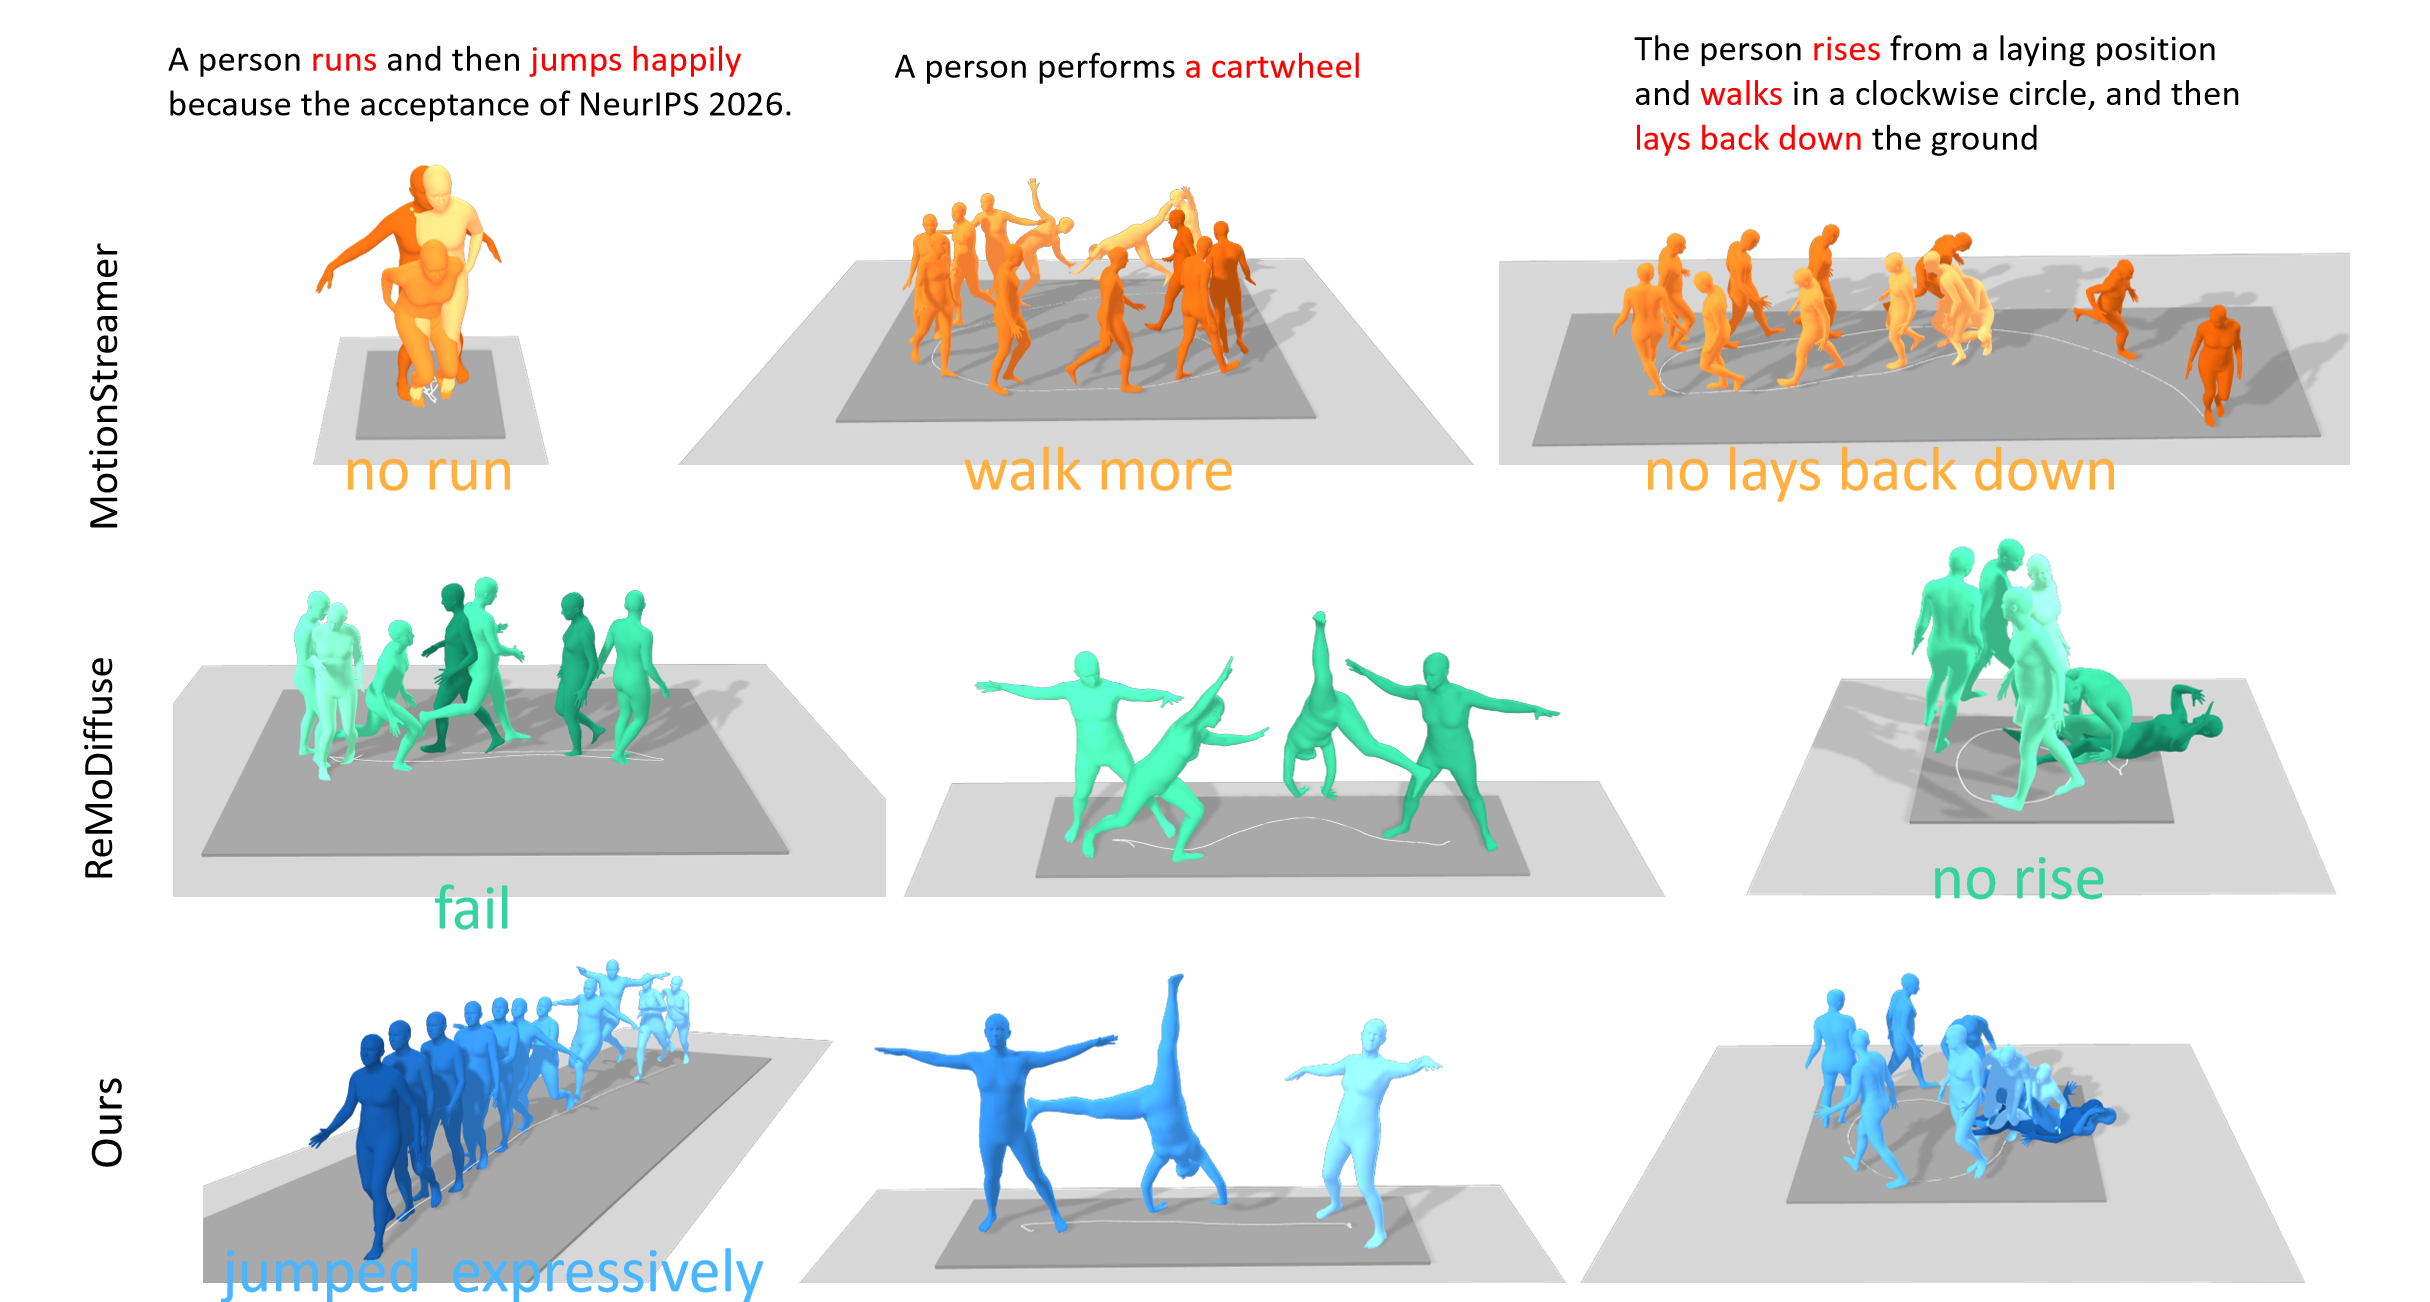
\includegraphics[width=\textwidth]{vis_v2.png}
  \caption{Qualitative comparison on challenging compositional text prompts. Each motion is rendered as a sequence of SMPL meshes with a light-to-dark color gradient indicating temporal progression. Compared to MotionStreamer and ReMoDiffuse, MSA-T2M produces motions with more accurate action ordering, correct body-part coordination, and smoother transitions between action phases.}
  \label{fig:vis}
\end{figure*}

Fig.~\ref{fig:vis} shows side-by-side visual comparisons on three challenging compositional text prompts (e.g., sequences involving multi-stage actions or fine-grained body-part control).
MSA-T2M generates motions with correct action ordering and natural transitions, whereas MotionStreamer~\citep{xiao2025motionstreamer} frequently produces semantic drift in the later frames and ReMoDiffuse~\citep{zhang2023remodiffuse} exhibits pose artifacts at action boundaries.
These qualitative gains are consistent with the quantitative FID improvement and reflect the benefit of multi-scale semantic alignment in organizing the latent space for generation.
Additional comparisons are provided in the supplementary material.


\subsection{Ablation Studies}

We conduct ablations to validate each design choice in MSA-T2M.
All ablations use \(K{=}3\) for efficiency; the main SOTA comparison uses \(K{=}5\) (see paragraph below).

\textbf{Component ablation.}
Tab.~\ref{tab:ablation} dissects the contributions of local alignment, global alignment, and retrieval augmentation.

\begin{table*}[t]
\centering
\caption{Component ablation on HumanML3D-272 (TMR protocol, $K{=}3$). Best in \textbf{bold}, second best \underline{underlined}.}
\label{tab:ablation}
\begin{tabular}{lcccccc}
\toprule
Methods & FID $\downarrow$ & R@1 $\uparrow$ & R@2 $\uparrow$ & R@3 $\uparrow$ & MM-D $\downarrow$ & Div $\rightarrow$ \\
\midrule
Real motion & 0.002 & 0.702 & 0.864 & 0.914 & 15.151 & 27.492 \\
\midrule
w/o local align, w/o RAG (global only) & \underline{11.306} & \underline{0.639} & 0.802 & \underline{0.864} & \underline{15.925} & 27.207 \\
w/o global align, w/o RAG (local only) & -- & -- & -- & -- & -- & -- \\
w/o RAG (local + global align) & 11.767 & 0.647 & \underline{0.805} & 0.842 & 15.983 & \underline{27.442} \\
w/o local align (global align + RAG) & 11.428 & \textbf{0.649} & \textbf{0.816} & \textbf{0.886} & \textbf{15.784} & 27.165 \\
Ours (local + global + RAG) & \textbf{10.896} & 0.637 & 0.794 & 0.859 & 16.030 & \textbf{27.336} \\
\bottomrule
\end{tabular}
\end{table*}

\textit{(1) RAG consistently improves motion quality.}
Removing the RAG branch while keeping both alignment losses (``w/o RAG'') increases FID from 10.896 to 11.767 (+0.871, $+$8.0\%).
This confirms that real motion priors from the semantically structured prior bank provide complementary guidance beyond text conditioning alone, and that alignment alone is insufficient to reach the best FID.

\textit{(2) Local alignment is the primary driver of latent space structure.}
Global alignment alone (``w/o local align, w/o RAG'') achieves FID~11.306, which already outperforms the model without any alignment (represented approximately by pure MotionStreamer at 11.790), indicating that even coarse global alignment improves the latent space.
However, the variant retaining global alignment and RAG but removing local alignment (``w/o local align'') achieves FID~11.428---worse than our full model by 0.532---demonstrating that frame-level supervision from BABEL is essential for fine-grained semantic structure in the latent space.

\textit{(3) Global alignment amplifies retrieval benefit.}
The full model (10.896) outperforms ``w/o local align'' (11.428) despite both having retrieval.
The difference traces to the quality of \(\mathbf{h}_{\text{cls}}\) as a retrieval key: with both local and global alignment, \(\mathbf{h}_{\text{cls}}\) captures compositionally-aware sequence semantics, producing more relevant retrieved priors.
Global alignment thus amplifies retrieval gain---a synergy that neither component achieves in isolation.

\textit{(4) Full model achieves best FID and Diversity.}
The complete MSA-T2M achieves best FID (10.896) and best Diversity (27.336), validating that multi-scale alignment and RAG are jointly necessary for optimal motion quality and coverage.
The slight decrease in R-Precision relative to ``w/o local align'' is expected: local alignment regularizes the latent space toward diverse action semantics, which can reduce retrieval recall while improving generation realism.

\textbf{Effect of retrieved sample count \textit{K}.}
Fig.~\ref{fig:ablation_k} shows that FID improves from \(K{=}1\) to \(K{=}5\) (best FID) but degrades beyond \(K{=}7\), while R@3 remains stable throughout.
This indicates that a moderate number of priors provides sufficient semantic coverage without introducing out-of-distribution noise; we fix \(K{=}5\) for SOTA comparison and \(K{=}3\) for ablations.

\begin{figure}[t]
\centering
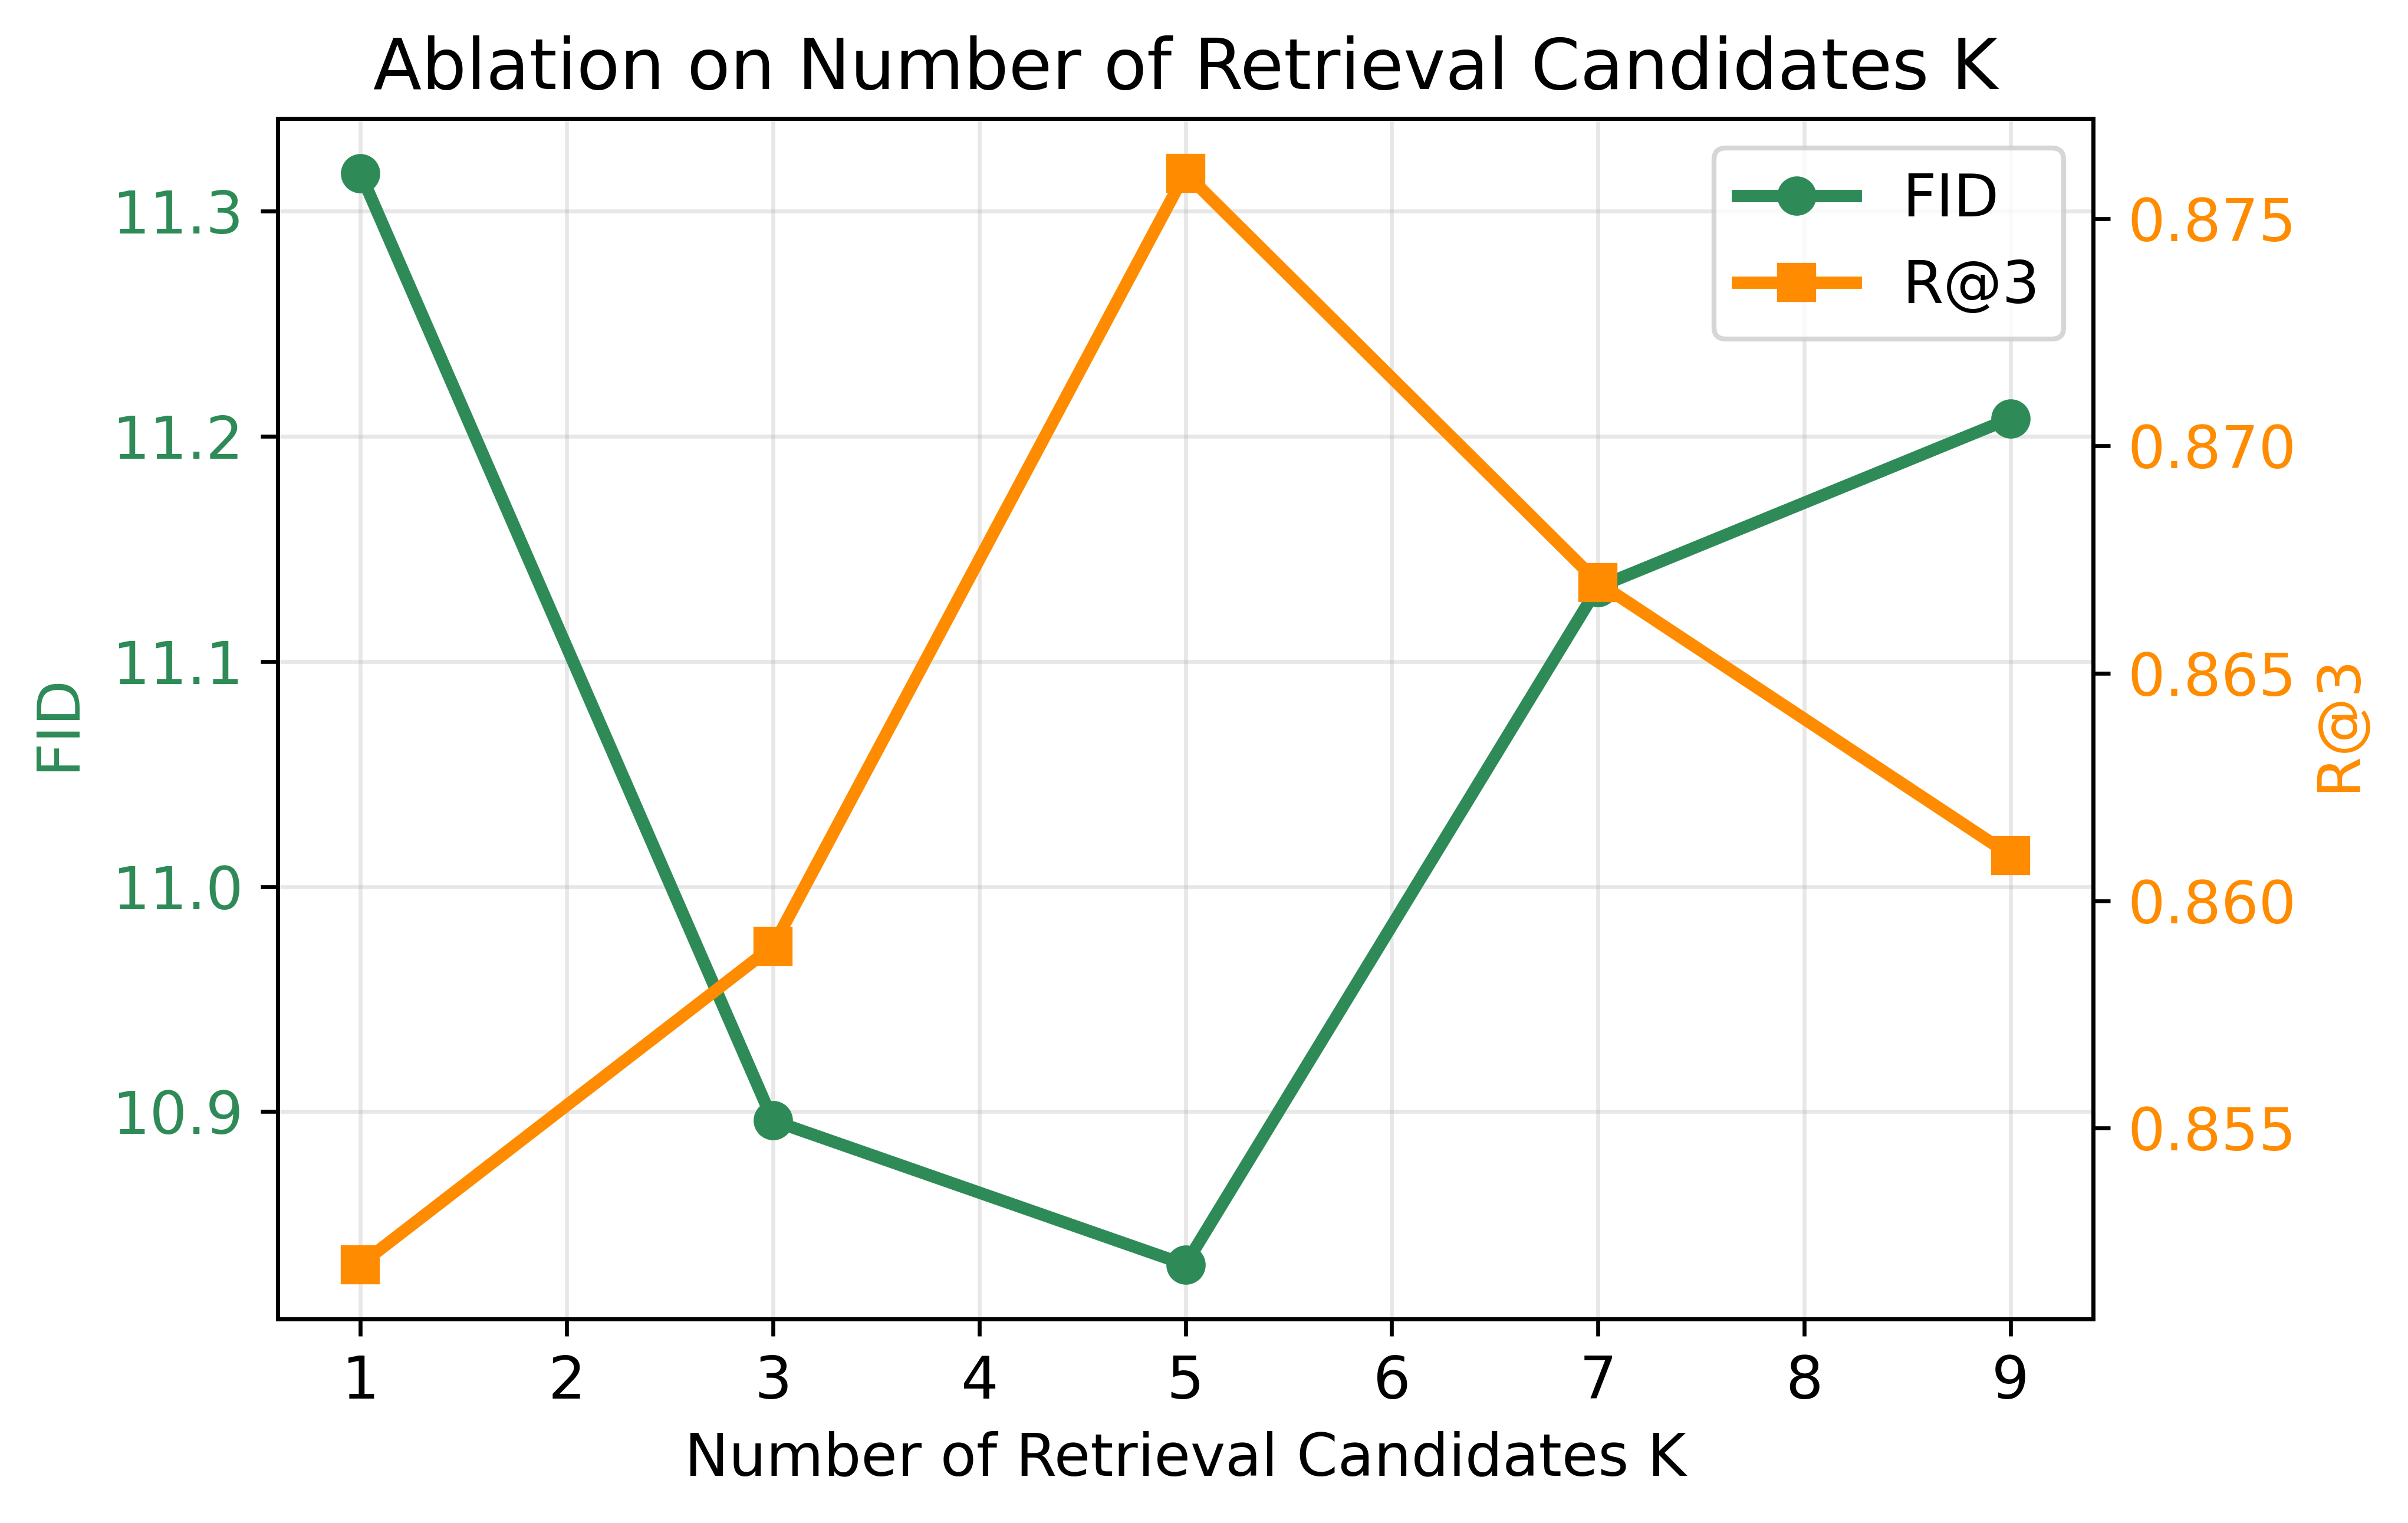
\includegraphics[width=\linewidth]{ablation_k_fid_r3.png}
\caption{Effect of retrieved sample count $K$ on FID and R@3. FID is minimized at $K{=}5$; R@3 is relatively insensitive to $K$.}
\label{fig:ablation_k}
\end{figure}




\section{Conclusion and Limitation}
In this work, we propose MSA-T2M, a text-driven motion generation model that for the first time achieves multi-scale semantic alignment in a continuous causal latent space and fully exploits the dividends of alignment via a retrieval-augmented generation (RAG) mechanism, enabling high-quality autoregressive diffusion motion synthesis. By exploring hierarchical latent space modeling together with semantic alignment, our method produces realistic and natural motions that more faithfully follow text instructions, achieving state-of-the-art results on a range of metrics including FID and R-Precision. An important finding is that simultaneously introducing both local and global multi-scale semantic alignment in the latent space yields a ``1+1>2'' synergistic effect: it generates more realistic motions while maintaining competitive text-motion retrieval accuracy. Furthermore, we observe that appropriately incorporating motion latent priors to guide autoregressive diffusion generation improves both realism and semantic fidelity, confirming the positive role of external knowledge injection in generation quality.


Despite its strong performance, MSA-T2M has several limitations. First, current datasets with frame-level action labels (e.g., BABEL) only describe atomic actions such as ``walk'', ``turn'', ``stand'', and ``sit'', lacking fine-grained annotations of specific body-part behaviors (e.g., ``a person raises their right hand and waves it three times'' instead of simply ``wave''). This makes it difficult for the model to precisely follow complex instructions that involve detailed body-part control. In the future, we plan to leverage large language models to construct richly annotated datasets and design more advanced architectures to achieve higher-precision text-to-motion generation, moving the model toward industrial-ready applications. Second, the current model supports only offline single-segment motion generation with a length limited by the training data. Extending multi-scale semantic alignment to online streaming motion generation and further unleashing the power of motion latent priors to produce natural, realistic, and infinitely long motions is an exciting direction for future work.



\begin{ack}
Use unnumbered first level headings for the acknowledgments. All acknowledgments
go at the end of the paper before the list of references. Moreover, you are required to declare
funding (financial activities supporting the submitted work) and competing interests (related financial activities outside the submitted work).
More information about this disclosure can be found at: \url{https://neurips.cc/Conferences/2026/PaperInformation/FundingDisclosure}.


Do {\bf not} include this section in the anonymized submission, only in the final paper. You can use the \texttt{ack} environment provided in the style file to automatically hide this section in the anonymized submission.
\end{ack}

\section*{References}


References follow the acknowledgments in the camera-ready paper. Use unnumbered first-level heading for
the references. Any choice of citation style is acceptable as long as you are
consistent. It is permissible to reduce the font size to \verb+small+ (9 point)
when listing the references.
Note that the Reference section does not count towards the page limit.
\medskip


{
\small


[1] Alexander, J.A.\ \& Mozer, M.C.\ (1995) Template-based algorithms for
connectionist rule extraction. In G.\ Tesauro, D.S.\ Touretzky and T.K.\ Leen
(eds.), {\it Advances in Neural Information Processing Systems 7},
pp.\ 609--616. Cambridge, MA: MIT Press.


[2] Bower, J.M.\ \& Beeman, D.\ (1995) {\it The Book of GENESIS: Exploring
  Realistic Neural Models with the GEneral NEural SImulation System.}  New York:
TELOS/Springer--Verlag.


[3] Hasselmo, M.E., Schnell, E.\ \& Barkai, E.\ (1995) Dynamics of learning and
recall at excitatory recurrent synapses and cholinergic modulation in rat
hippocampal region CA3. {\it Journal of Neuroscience} {\bf 15}(7):5249-5262.
}


%%%%%%%%%%%%%%%%%%%%%%%%%%%%%%%%%%%%%%%%%%%%%%%%%%%%%%%%%%%%

\appendix

\section{Technical appendices and supplementary material}
Technical appendices with additional results, figures, graphs, and proofs may be submitted with the paper submission before the full submission deadline (see above). You can upload a ZIP file for videos or code, but do not upload a separate PDF file for the appendix. There is no page limit for the technical appendices. 

Note: Think of the appendix as ``optional reading'' for reviewers. The paper must be able to stand alone without the appendix; for example, adding critical experiments that support the main claims to an appendix is inappropriate. 

%%%%%%%%%%%%%%%%%%%%%%%%%%%%%%%%%%%%%%%%%%%%%%%%%%%%%%%%%%%%

\newpage
\input{checklist.tex}

\bibliographystyle{plainnat}
\bibliography{mybib}


\end{document}